\documentclass[twocolumn]{article}

\usepackage{fullpage}
\usepackage{graphicx}

\title{Identifying Notes in Recorded Music Using a Naive Bayes Classifier}
\date{April 25, 2011}
\author{Author}

\begin{document}

\maketitle

\begin{abstract}
A method for detecting notes present in an audio recording is implemented and tested.  The audio data is analyzed in the frequency domain in order to obtain intuitive features.  The audio data is split into many small frames in order to obtain analyses for multiple small periods of time.  A Naive Bayes classifier is used to classify the features thus obtained.  The performance of this classifier is evaluated; accuracy varies from 65\% in the worst case to 80\% in the best.  Promising avenues for significant further improvement are outlined.
\end{abstract}

\section*{Keywords}
Transcription, Naive Bayes, Music, Audio

\section{Introduction}

Musical transcription is the process of identifying the notes which are played to produce the sound which is heard.  When performed by humans, it is laborious and requires significant musical training.  It would be very helpful if this task could be automated.  Even if automated transcription cannot provide perfect accuracy, a good first approximation which can be refined manually would be useful.

The fundamental problem which needs to be solved in order to transcribe music can be phrased as the following question: ``At a given time, is a given note being played?''.  If this question can be answered accurately, transcription is straightforward.

A musical note is the sound produced by the resonance of a musical instrument.  A real musical instrument will resonate at multiple frequencies, all of which are members of the harmonic set defined by some fundamental frequency.  A note is identified by its pitch, which is in turn defined by fundamental frequency alone.  The higher harmonics of the fundamental frequency determine the timbre of the note, but do not contribute to its identity.

\begin{figure}[htb]
  \centering
  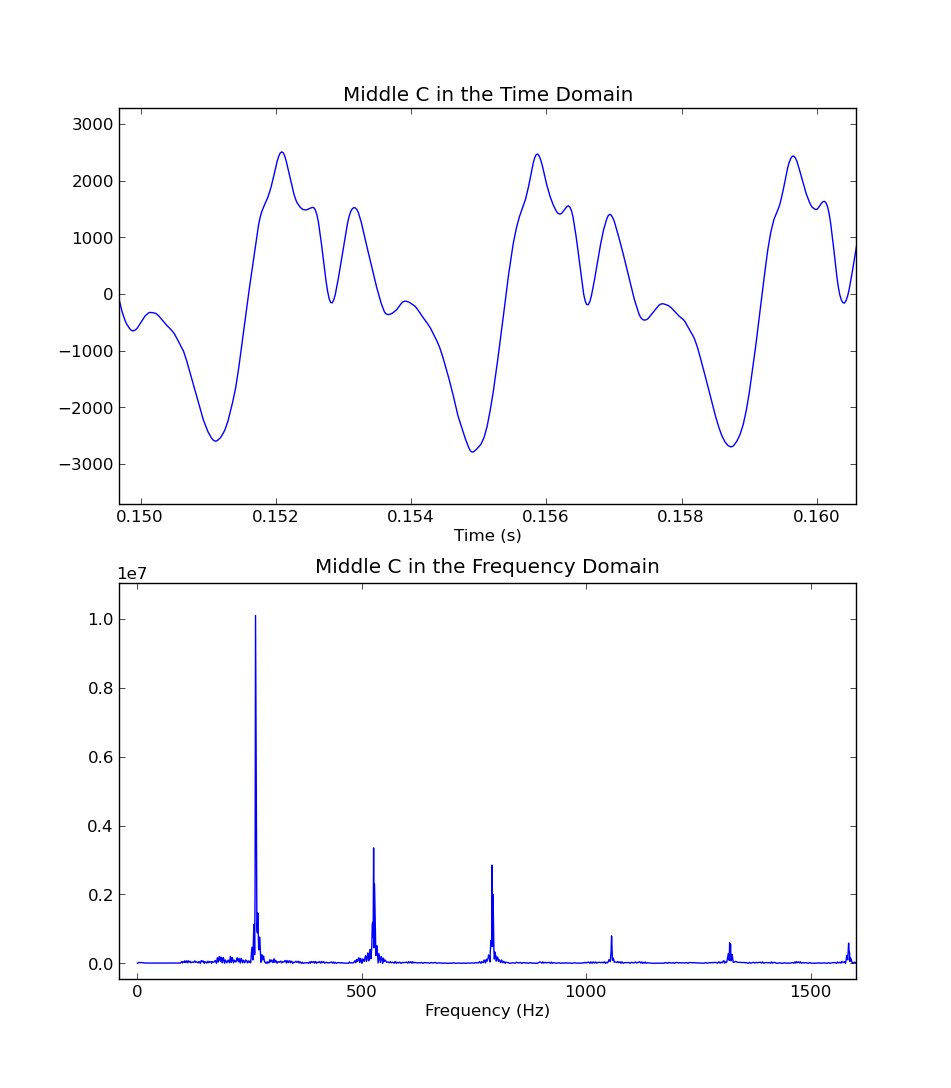
\includegraphics[scale=0.335]{middlec.png}
  \caption{Middle C shown in both the frequency and time domain}
  \label{middlec}
\end{figure}

Figure \ref{middlec} shows a single note in both the frequency and time domain.  The time domain signal is a fairly simple periodic function; it is clear that we could measure the fundamental frequency in the time domain, identifying the note.  The fourier transform of the signal is even simpler; the fundamental frequency is identifiable as the first peak, and subsequent peaks are visible for each harmonic.

Determining which notes are being played at a given time in a signal means distinguishing between fundamental frequencies and harmonic frequencies.  For the case of a single note, as shown in Figure \ref{middlec}, this is very simple.  This task is complicated significantly when multiple notes are present in the signal.

\begin{figure}[htb]
 \centering
 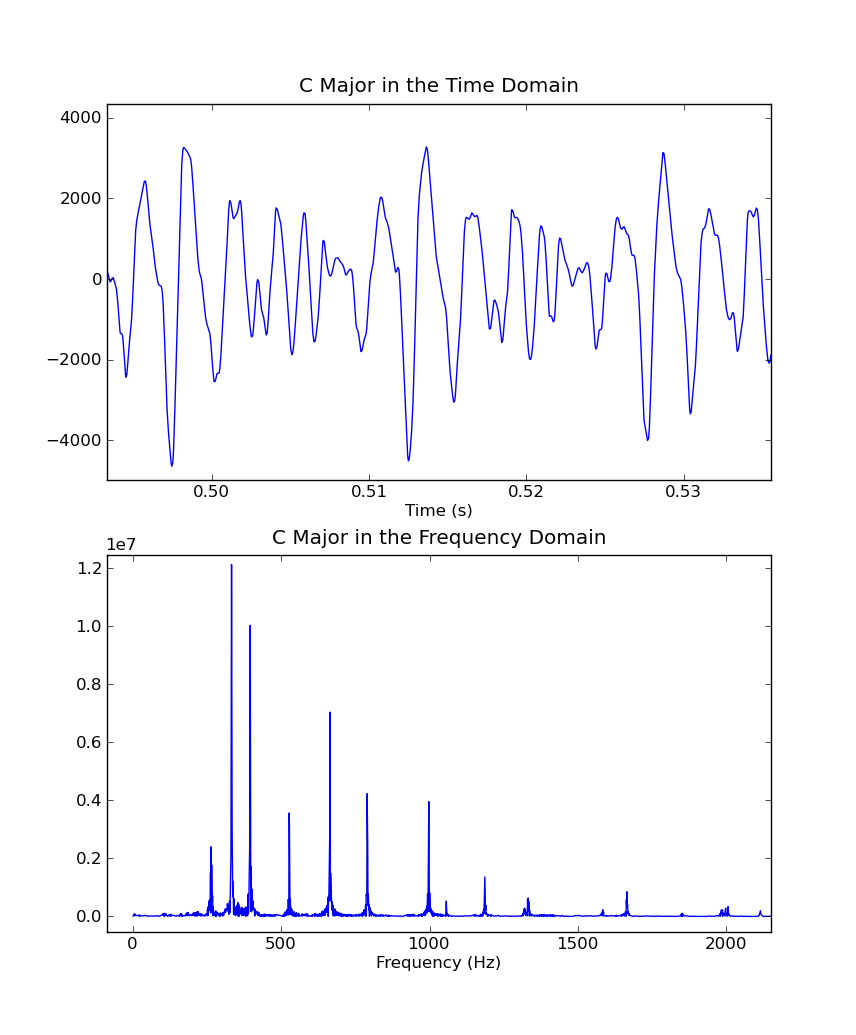
\includegraphics[scale=0.37]{cmajor.png}
 \caption{C Major chord in both the frequency and time domain}
 \label{cmajor}
\end{figure}

Figure \ref{cmajor} shows the C Major chord played in standard form, in the frequency and time domain.  It is composed of three individual notes.  Some periodicity is visible in the time domain signal, but it is difficult to imagine an effective time domain method for identifying the three notes which are sounding.  The frequency domain, on the other hand, presents fairly simple data.  Since each note is composed of a series of impulses in the frequency domain, the fourier transform of multiple simultaneous notes is also a series of impulses.  In the case of a simple major triad, no fundamental frequency overlaps an overtone of another note, so it is trivial to identify the fundamental frequencies: they are the impulses whose frequencies are not multiples of the frequencies of any other impulses.

Clearly, it is possible to procedurally identify multiple notes so long as no fundamental frequency coincides with a harmonic of another fundamental frequency.  Note identification only becomes an interesting separation problem if some notes lie on other notes' overtones.  This raises an obvious question: in real music, how often are notes which are overtones of other notes played?

Qualitatively, human perception of the harmony of multiple notes is essentially a measure of the degree of coincidence of the notes' harmonic frequencies.  Since music is generally intended to be in harmony, this suggests that one should expect significant collision between the harmonic series present at any time.

More quantitatively, the fundamental frequencies of notes in the western scale can be described by the formula:

\begin{equation}
F_i = F_R \cdotp 2^{\frac{i}{12}}
\label{scale}
\end{equation}

Where $i$ is an integer representing the number of semitones of separation from the reference note.  The harmonic series of a given frequency is simply a sequence of multiples of the fundamental frequency:

\begin{equation}
[F_o, 2 \cdotp F_o, 3 \cdotp F_o, \cdots]
\label{harmonicseries}
\end{equation}

(\ref{harmonicseries}) is approximately equal to the following:

\begin{equation}
[F_o, F_o \cdotp 2^{\frac{12}{12}}, F_o \cdotp 2^{\frac{19}{12}}, F_o \cdotp 2^{\frac{24}{12}}, F_o \cdotp 2^{\frac{28}{12}}, \cdots]
\label{harmonicseries2}
\end{equation}

Inspecting (\ref{harmonicseries2}), it can be seen that the overtones of a note fall on its octave, then its major fifth, then the second octave, then a major third, and so on.  The overtones of the note fall upon other notes in the major chord, in octaves above the note.  Since major intervals are extremely common in real music, it follows that it is very likely that notes will be played coinciding with the overtones of lower notes.

\begin{figure}[htb]
 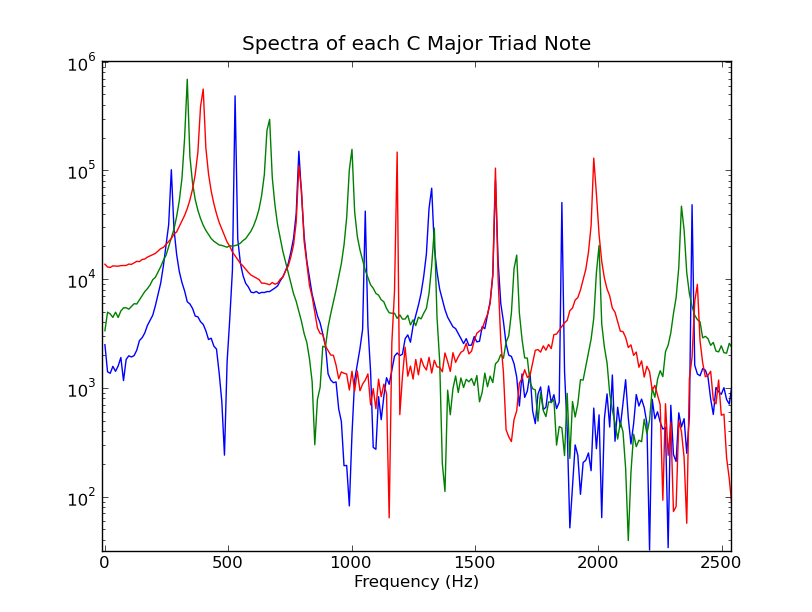
\includegraphics[scale=0.39]{cmajor-decomp.png}
 \caption{Frequency domains of notes present in the C major triad}
 \label{cmajor-decomp}
\end{figure}

Figure \ref{cmajor-decomp} provides an illustration of how notes' harmonic series collide.  Note the peaks common to different notes in the major triad.  Also, it is very important to observe that all of the peaks visible in this figure correspond to higher notes which belong to other forms of the same major chord.

\section{Proposed Technique}

In order to solve the problem, an algorithm is required which can determine whether or not a given note is present in an audio signal.  If a note is present in the signal, a peak will exist in the frequency domain at the fundamental frequency of the note, and this peak will not be the sole product by a harmonic of a lower frequency.

In order to obtain a representation of the frequency domain within a limited slice of time, the audio signal is divided into a multitude of small frames.  The discrete fourier transform of each frame is computed, providing an estimate of the frequency domain for the duration of the frame.  The frequency domain of the frame is to be evaluated in order to determine whether or not a given note is sounding in that frame.

Two features are proposed in order to address the identification of peaks at the fundamental frequency of the note.

The first is peak magnitude, which is simply the highest magnitude among frequencies near the note's nominal fundamental, relative to the average signal level.  Searching a small region surrounding the the nominal fundamental gives this metric the ability to tolerate notes which are slightly out of tune.  Measuring the magnitude of the maximum relative to the average signal level is intended to eliminate the effect of signal gain.

The second feature is the second derivative with respect to frequency at the maximum used for the first metric.  A fundamental frequency appears as an impulse in the frequency domain. This metric is intended to evaluate whether the maximum found for the first feature represents a plausible impulse function.  The second derivative is proportional to the rate of curvature of the frequency domain signal; it will be very high if the signal is impulsive.  This feature should reject local maxima which arise as a result of spectral bleed.  As with the first feature, the second derivative is scaled by the average signal level, in order to reduce the effect of gain.

In order to differente fundamental frequencies from harmonic frequencies, a third and final feature is introduced.  This feature is the difference between the peak magnitude for the current note, and the largest peak magnitude among lower frequencies which could produce the current note's frequency as a harmonic.  The magnitudes of fundamental frequencies are expected to be large relative to harmonics.  If both a harmonic and a fundamental exist at a note's frequency, the magnitude of the fundamental will be added to the magnitude of the harmonic, yielding a large magnitude relative to lower fundamentals.  Conversely, if no fundamental exists at the note, then the magnitude of a peak at the note can be expected to be small relative to lower fundamentals.

\begin{figure}
 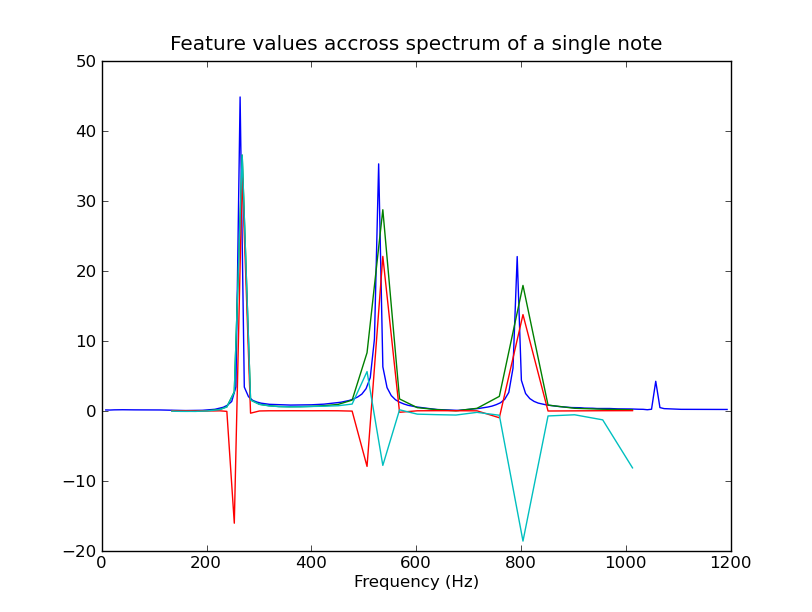
\includegraphics[scale=0.39]{features.png}
 \caption{Feature values for all notes, accross the spectrum of a single note.  Blue is the frequency domain signal.  Green is the peak magnitude.  Red is the second derivative.  Cyan is ratio of peak magnitude to potential fundamental peak magnitude}
 \label{features}
\end{figure}

Figure \ref{features} shows how the described features behave in the simple case of a single note.  All three features have large magnitudes for the fundamental frequency.  Peak magnitude and the second derivative are both large for the harmonic peaks.  Note how the second derivative is negative and large for the elevated peak magnitude values for notes adjacent to peaks, which arise due to spectral bleed.  Finally, note how the difference between peak magnitude and lower harmonic peak magnitude is negative for the harmonic peaks.

It is possible to classify these features using a Naive Bayes classifier.  Naive Bayes is quite simple to implement, since the problem provides binary hypothesis: either the note is sounding, or it is not.  Feature probabilities are estimated by assuming that features belonging to either hypothesis have a gaussian distribution.  The mean and variance of each feature are calculated from learning data.

\section{Experiments and Results}

The classification method was tested with a variety of structured piano recordings.  A number of types of recordings were used:

\begin{itemize}
 \item Single notes \\
 \item Major triads \\
 \item Octaves \\
 \item Major triads, with octave \\
 \item Two major triads \\
\end{itemize}

The single notes are intended as a baseline, simplest case test of the classifier.  These test cases should be easy to classify, but are not representative of any but the simplest of music.

The major triads are another simple case.  They introduce additional harmonics, as well as worsening spectral bleed effects by placing notes closer together.  These are common in music, but are still a fairly simple case.  No fundamentals collide with the harmonics of other notes, although some harmonics are common to multiple notes.

The octaves, which are the combination of a note and its octave, are intended to represent the simplest possible case of a fundamental frequency colliding with a harmonic.  The fundamental of the octave is the first harmonic of the root note.  All harmonics of the octave collide with harmonics of the root.

The major triads with octaves consist of a major triad, combined with the root played one octave down.  This combines the harmonic complexities present in the major triad with the collisions between triad fundamentals and and harmonics of the lower octave.

The two major triads are played one octave separate.  This is intended to provide a pathological case, since each note in the upper triad collides with the harmonics of at least one note in the lower triad.  Numerous harmonic peaks exist, and harmonic sets coincide frequently.

Together, these test cases are expected to be representative of the types of interactions between notes which are common in music.  Each test case consists of several seconds of recorded audio, including attack transients and significant decay.  Each test case is played manually, with variance in note volume accross the dataset.  The single note and major triad test sets consist of twenty-five test cases, covering two complete octaves.  The octave, octave-major, and two-major test sets each include thirteen test cases, covering one complete octave.  Since the content of each test case is well known, all of these test cases can easily be labelled.  From these test cases, a total of 6930 positive features and 34650 negative features are available.  `Positive Features' are features representing notes which are known to be sounding, `Negative Features' are features representing notes which are known not to be sounding.

The performance of the Naive Bayes classifier is evaluated for each of the test datasets alone, as well as for all of the datasets combined.  In all cases, labelled data was randomly divided into the training and testing feature sets.

\begin{table}[htb]
\centering
\begin{tabular}{|l|c|c|}
\hline
Dataset & Positive & Negative \\
\hline
Notes & 84.5\% & 94.9\% \\
\hline
Majors & 71.6\% & 93.8\% \\
\hline
Octaves & 72.1\% & 94.6\% \\
\hline
Octave-Majors & 76.4\% & 94.9\% \\
\hline
Two Majors & 65.1\% & 94.0\% \\
\hline
All & 66.4\% & 93.0\% \\
\hline
\end{tabular}
\caption{Naive Bayes learning accuracies}
\label{learning}
\end{table}

Table \ref{learning} shows the accuracies of the Naive Bayes classifier when classifying the training data.  Positive accuracy is the proportion of positive features which are classified correctly, and is the complement of the false negative rate of the classifier.  Negative accuracy is the proportion of negative features which are classified correctly, and is the complement of the false positive rate of the classifier.

The accuracy of the Naive Bayes classifier when classifying the testing data is shown in Table \ref{testing}

\begin{table}[htb]
\centering
\begin{tabular}{|l|c|c|}
\hline
Dataset & Positive & Negative \\
\hline
Notes & 80.8\% & 95.4\% \\
\hline
Majors & 71.1\% & 94.1\% \\
\hline
Octaves & 67.6\% & 93.2\% \\
\hline
Octave-Majors & 75.5\% & 94.0\%  \\
\hline
Two Majors & 64.7\% & 93.5\%  \\
\hline
All & 64.8\% & 93.4\%  \\
\hline
\end{tabular}
\caption{Naive Bayes testing accuracies}
\label{testing}
\end{table}

\section{Conclusions}
The observed accuracies are quite encouraging. It is interesting to observe that the false positive rate is much lower than the false negative rate, and that the false positive rate remains essentially the same for all test types.

It is likely that the assumption that features have gaussian distributions is not particularly accurate.  The negative features, in particular, are likely to be multimodal, with separate clusters for notes which have no peaks at all, and for notes which coincide with harmonics of other notes.  It is expected that the presence of multiple modes results in a high variance, which skews classification in favour of the negative hypothesis.  This explains the high false negative and low false positive rate observed in testing.

This flaw yields an obvious avenue for improvement:  If feature distributions are indeed multimodal, the probability estimation method should be modified to be able to accomodate this distribution.  Negative and positive labelled data might be separated into clusters by K-means, and Naive Bayes used to evaluate the most probable cluster for a feature.  Alternatively, hypothesis probability might be estimated in a non-parametric way using Parzen Windowing.

Another significant source of inaccuracy is in the use of the discrete fourier transform to obtain an estimate of the frequency domain.  Note frequencies rise exponentially (see Equation \ref{scale}), and discrete fourier transform frequencies rise linearly.  This means that the discrete fourier transform provides better resolution for higher notes than lower: every octave, the number of frequency data points between notes doubles.

\begin{table}[hbt]
 \centering
 \begin{tabular}{|l|c|c|}
  \hline
  Dataset & Positive & Negative \\
  \hline
  Low Majors & 60.8\% & 91.3\% \\
  \hline
  High Majors & 88.8\% & 94.9\% \\
  \hline
 \end{tabular}
 \caption{Major chord testing accuracy for low and high major chords}
 \label{frequencyeffect}
\end{table}

Table \ref{frequencyeffect} shows classification accuracy for the highest and lowest six major chord test cases.  Classification accuracy for the highest chords is substantially greater than the classification accuracy of 71.1\% observed for the entire set, while the classification accuracy for the lowest chords is substantially lower than the accuracy for the entire set.

The only difference between the low and high test cases is that the frequency resolution relative to semitone distance is about three times larger for the high chords.  Clearly, classification accuracy is strongly dependent on frequency resolution, which stands to reason.

Performance could likely be greatly improved if frequency resolution could be increased.  Simply increasing the resolution of the discrete fourier transform is difficult, since an increase in resolution requires an increase in frame size, which means that time resolution is lost.  This limitation might be worked around by dividing data into multiple frame sets with different frame sizes: larger frames with higher frequency resolution could be used to evaluate hypotheses for low notes, while smaller frames with higher time resolution could be used to evaluate hypotheses for high notes.  Alternatively, the use of the discrete fourier transform could be discarded entirely in favour of a wavelet transform, which eliminates the time/frequency resolution trade off at the cost of greater computational complexity.

\section*{Source Code}
All project code and data are available from:

\underline{http://svn.ipeet.org/ipcode/notetranscriber/}

Code is written in Python, and requires the NumPy and Matplotlib libraries.

\end{document}
